\chapter{Results}\label{chap3}
\thispagestyle{plain}

As mentioned in Section \ref{chap2}, three machine learning algorithms have been trained, and the resulting models used to predict glaciers ice thickness. The same procedure has been applied to all the algorithm used, in order to compare the results between the different models. 
All the algorithm have been trained and tested using the data available in the GlaThiDa data-set in the alpine region. Only glaciers present in the GlaThiDa database belonging to Region 11 of the RGI (Central Europe) have been used in the following analysis.

After training each algorithm the resulting model has been used to predict the ice volume of all the glaciers in the alps. This is useful to compare the results of these model to those computed by \citet{Farinotti2019} in the third ITMIX.

\section{Results from Linear Regression}\label{linear}
The first model to be analyzed is the one obtained from training the linear regression algorithm. In order to assess how well a machine learning model makes predictions a sub-sample of the data-set is usually left out from the training process (see section \ref{training}). With the left out data the score from Eq. \ref{eq:score} is computed by letting the model predict the values not used for training. This is done to make sure the model is not over-fitted. Complex machine learning algorithm in fact might be very good at predicting data inside the training sample but might perform much worse on data outside this sample (over-fitting). 
This is usually not the case with linear regression, hence in principle there is no need to only use a sub-sample of the data to train the model. The $R^2$ coefficient (the score) could be computed using the whole data-set to train the model. The linear regression algorithm however, has been trained using the same procedure used for the other algorithms, to be able to better compare the models with each other, and try to find similarities and differences.     

\subsection{Score and volume spread}\label{lr-score}

\begin{figure}[!tp]
	\centering		  
	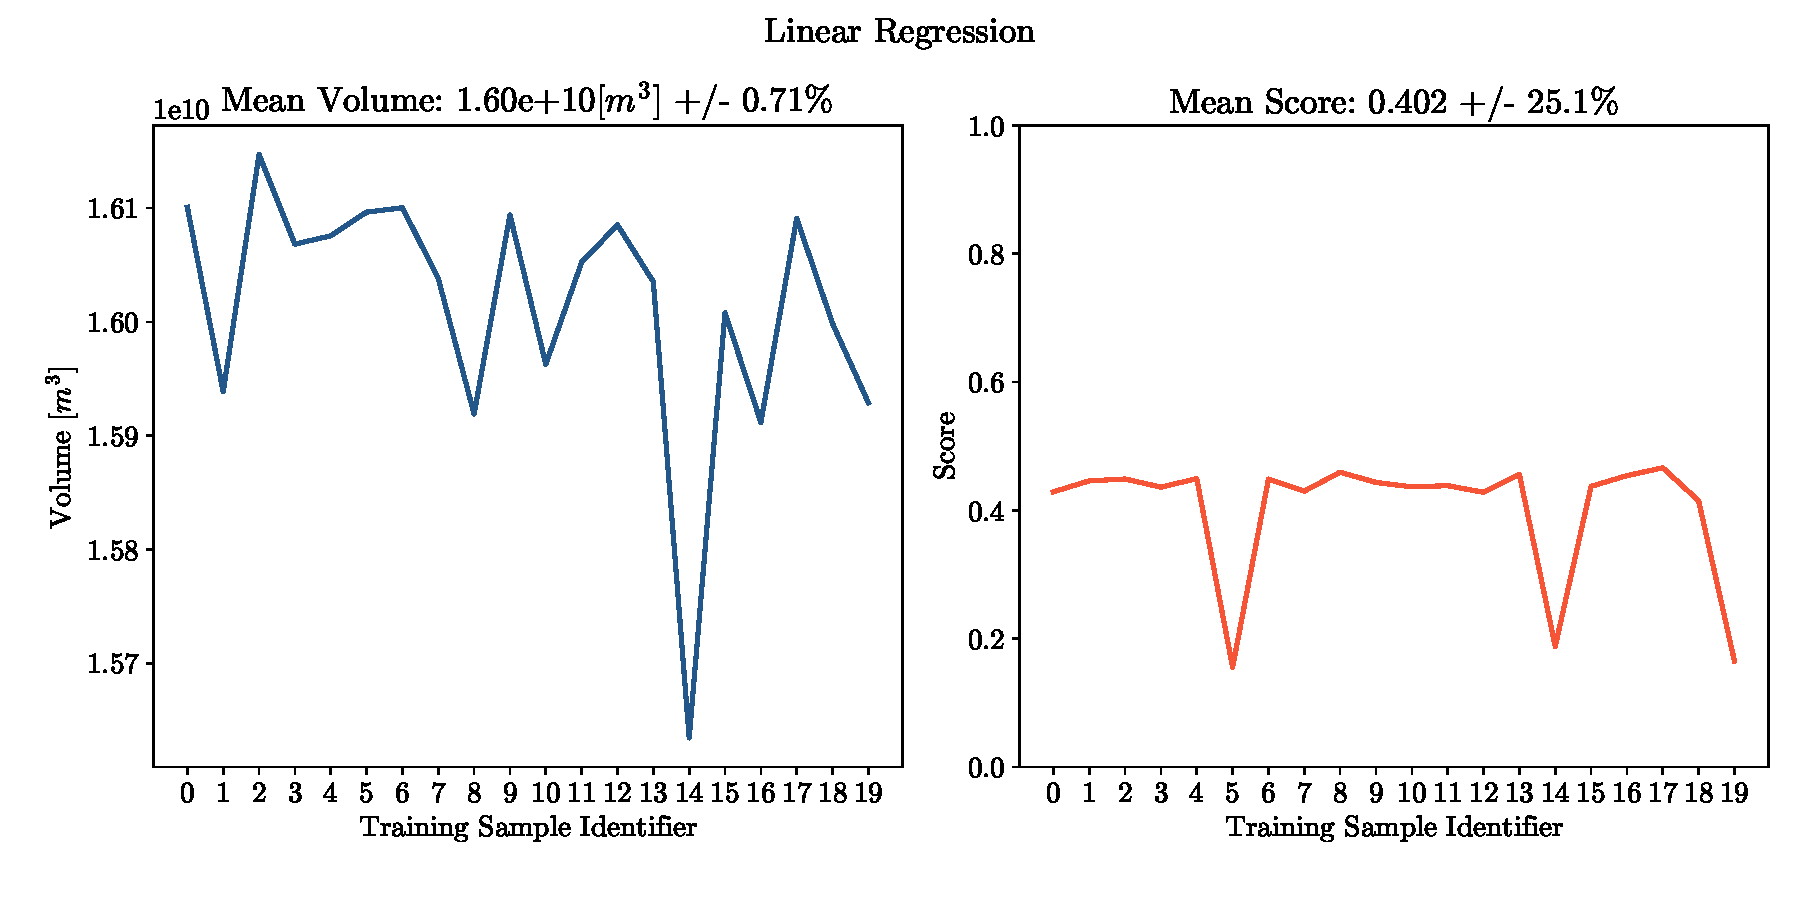
\includegraphics[width=1.\textwidth]{figures/LR_score.pdf}
	\caption{Linear Regression: Volume and score values of the model after training it with 20 different sub-sample of data. On the x-axis each number identifies a different sample of data. On the left the total volume of the alpine glaciers present in the GlaThiDa is shown. On the right the $R^2$ coefficient for values left out of the training sample.}
	\label{fig:lr-score}
\end{figure}

Figure \ref{fig:lr-score} shows the volume and score change  for 20 different sub-samples used to train the linear regression algorithm. Each number on the x-axis represents a different sample used for training: of all the alpine glaciers observations in the GlaThiDa, 75\% of them have been used for  training the model and the remaining 25\% to compute the score. 

The volume shown on the left side of Fig. \ref{fig:lr-score} has been computed on the full sample of alpine glaciers with ice thickness observations. Each value shown in the figure is obtained with a different model, derived from training it with the sub-samples. The mean volume for the 20 different sub-samples is $1.60\times 10^{10}$ $m^3$ with a relative standard deviation of 0.74\%. Sample 14 clearly predicts the lowest of all volumes.

\begin{figure}[!tp]
	\centering		  
	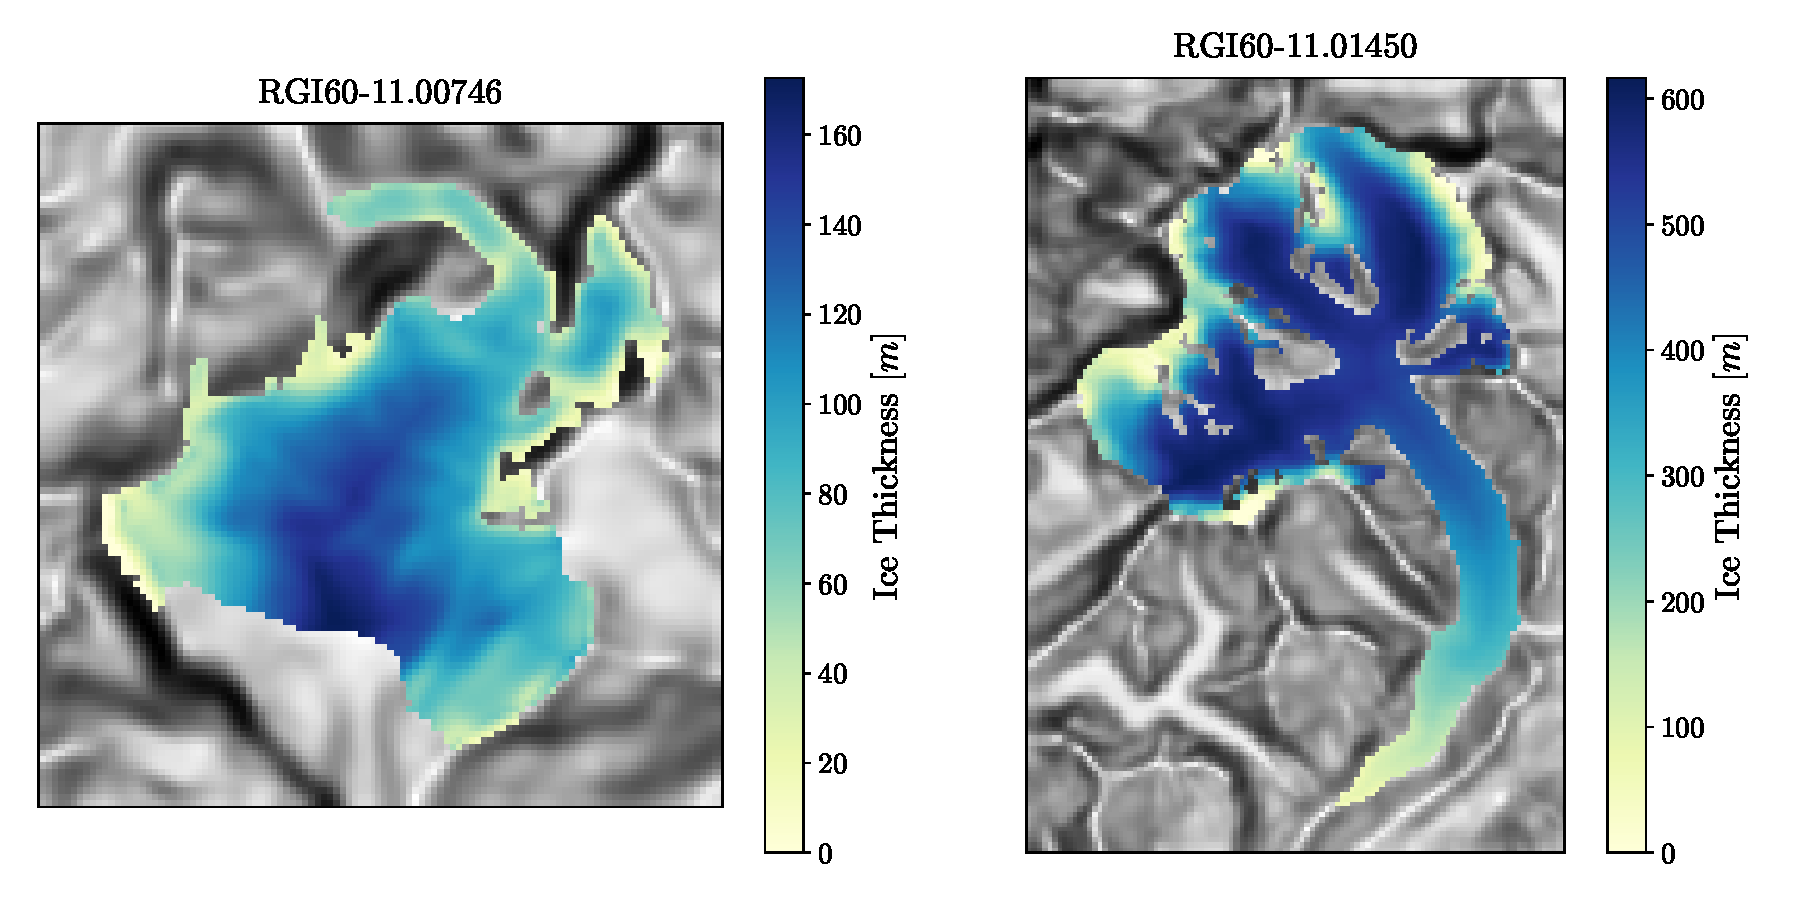
\includegraphics[width=1.\textwidth]{figures/LR_thick_map.pdf}
	\caption{Linear Regression: Ice thickness distribution for two glaciers on top of the terrain slope angle. On the left, one of the glaciers used to train the model. On the right, one of the glaciers outside those used to train the model.}
	\label{fig:lr-map}
\end{figure}

It is worth nothing that the model predicts ice thicknesses below zero for certain points. These have however been rounded to zero as a thickness below zero makes no physical sense.

The average score is 0.402 with a high 25.1\% relative standard deviation. Clearly this is due to the score dropping for sub-samples 5, 14 and 19. For most sub-samples the score is in fact above 0.4, but for those three it drops even below 0.2. Sub-sample 14 then leads to the lowest volume and a low score compared to the average.
The linear regression model trained with all the data in the data-set has score of 0.32 which  is the lowest among the three models used.

The total volume for the alps computed with the linear model is $1.40 \times 10^{11}m^3$ which is 9.8\% larger than the volume predicted by \citet{Farinotti2019}.

\subsection{Features Importance}  

It is interesting to look into which of the variables used to train the model influence the outcome of the prediction the most.

A very easy way to do so for a linear regression model, is just to analyze the weights $\bm{\beta}$ (see Eq. \ref{eq:linear}), which the model assigned to each feature in order to make predictions. These are shown in Table \ref{tb:lr-coef}.
The higher the absolute values of the coefficients, the more the variable will influence the outcome of the model. Looking at these coefficients, the slope angle is the feature which is more relevant to the outcome of the model, followed by the linear mass balance. In particular the slope influences the prediction almost 3 times more than the altitude and over 2.5 times more than the distance from the border. This means that a doubling of the slope angle of the glacier surface, will result in an ice thickness change 3 times larger than the change predicted by a doubling of the altitude. It is worth noting that the slope angle has a negative sign, meaning that lower slope angles correspond to higher ice thicknesses in accordance with the literature about glaciers ice flow \cite[P. 298]{cuffey2010physics}.

\begin{table}
	\centering
	\caption{Linear Regressions: Coefficients for the linear regression model: higher absolute values mean that the feature have a higher influence on the model predictions}
	\begin{tabular}{|c|c|c|c|}
		\hline 
		Slope Angle&Mass Balance&Distance From Border&Altitude \\
		\hline
		-19.7&12.7&7.7&-6.6 \\
		\hline
	\end{tabular}
	\label{tb:lr-coef}
\end{table}

The results form the coefficients analysis of the linear model, could be enough to have a complete picture about the variables influencing the output the most. An analysis showing the tools used for the other models is shown anyway, in order to have comparable results between the models, and to understand how these tools compare with the method of analyzing the magnitude of the linear model coefficients. 

Figure \ref{fig:lr-heatmap} shows the coefficients deriving from the permutation analysis explained in section \ref{permutation}. This looks at changes in the score of the model, when the feature values for a single feature are swapped around randomly. If the score doesn't change, compared to the one achieved by the model with the correct order of the features values, it would mean that the feature is less relevant in making predictions. The higher the permutation coefficient value, the more relevant is the feature in making predictions. Figure \ref{fig:lr-heatmap} shows that using this method the slope angle is the feature which most influences the outcome of the prediction, which is in accordance with the values of the model coefficients in table \ref{tb:lr-coef}. Also for the other features the permutation shows the same result already found with the model coefficients. Interestingly for sub-sample 5, 14 and 19, there is a significant drop in the permutation coefficient for all of the features. These were also the sub samples with the lowest score, registered in the score analysis for the linear regression model.

\begin{figure}[!tp]
	\centering		  
	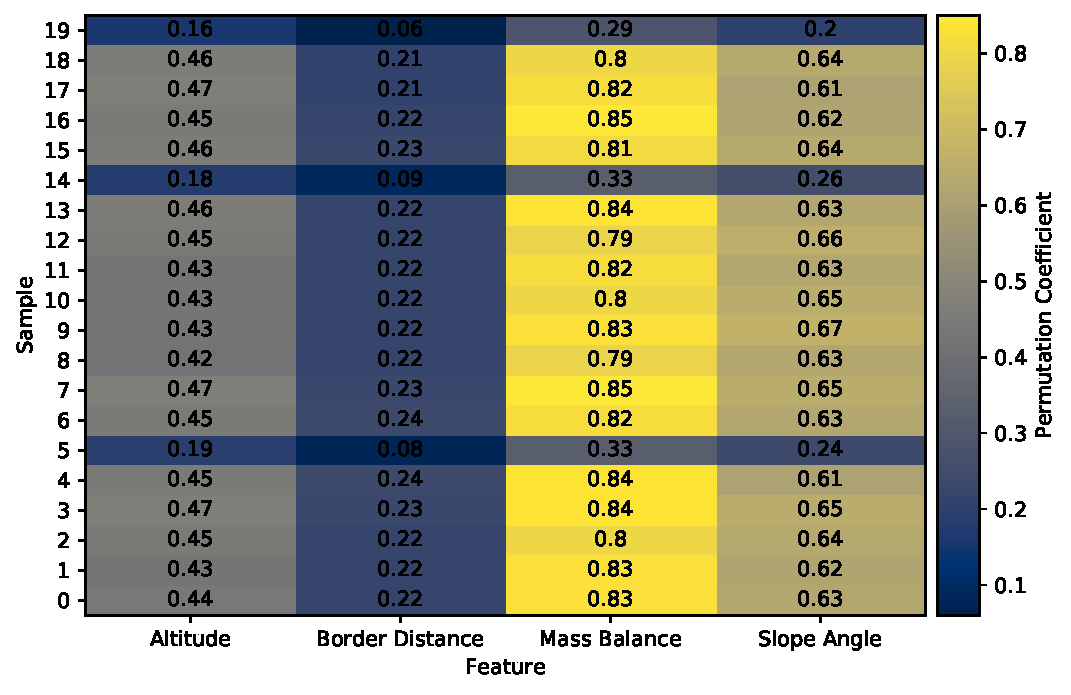
\includegraphics[width=1.\textwidth]{figures/LR_heatmap.pdf}
	\caption{Linear Regression permutation coefficients heatmap: each row in the figure represents a sub-sample of the data used for training the algorithm. Each column represents the permutation coefficient value for the considered feature.}
	\label{fig:lr-heatmap}
\end{figure}

Finally Fig. \ref{fig:lr-pdp} shows the change in thickness value for changes in values of the features. Features are scaled according to Eq. \ref{eq:scale}, hence the values on the x-axis of the figure do not represent the original input values, but the scaled ones used to train the model. Having scaled features helps reading this chart as features could have very different ranges and scales (for example altitudes ranging between  $2000m$ and almost $5000m$, compared to slope angles ranging from $0$ to $\frac{\pi}{4}$). Each line represents ice thickness changes when all other variables are kept constant. This provides for a visual comparison between the influence which each feature has on the prediction. For the linear regression case each line is a of course a straight line, but this will not be the case for the other models. Looking at the chart the same conclusions as for both the linear coefficient magnitude, and the permutation importance can be drawn.

\begin{figure}[!tp]
	\centering		  
	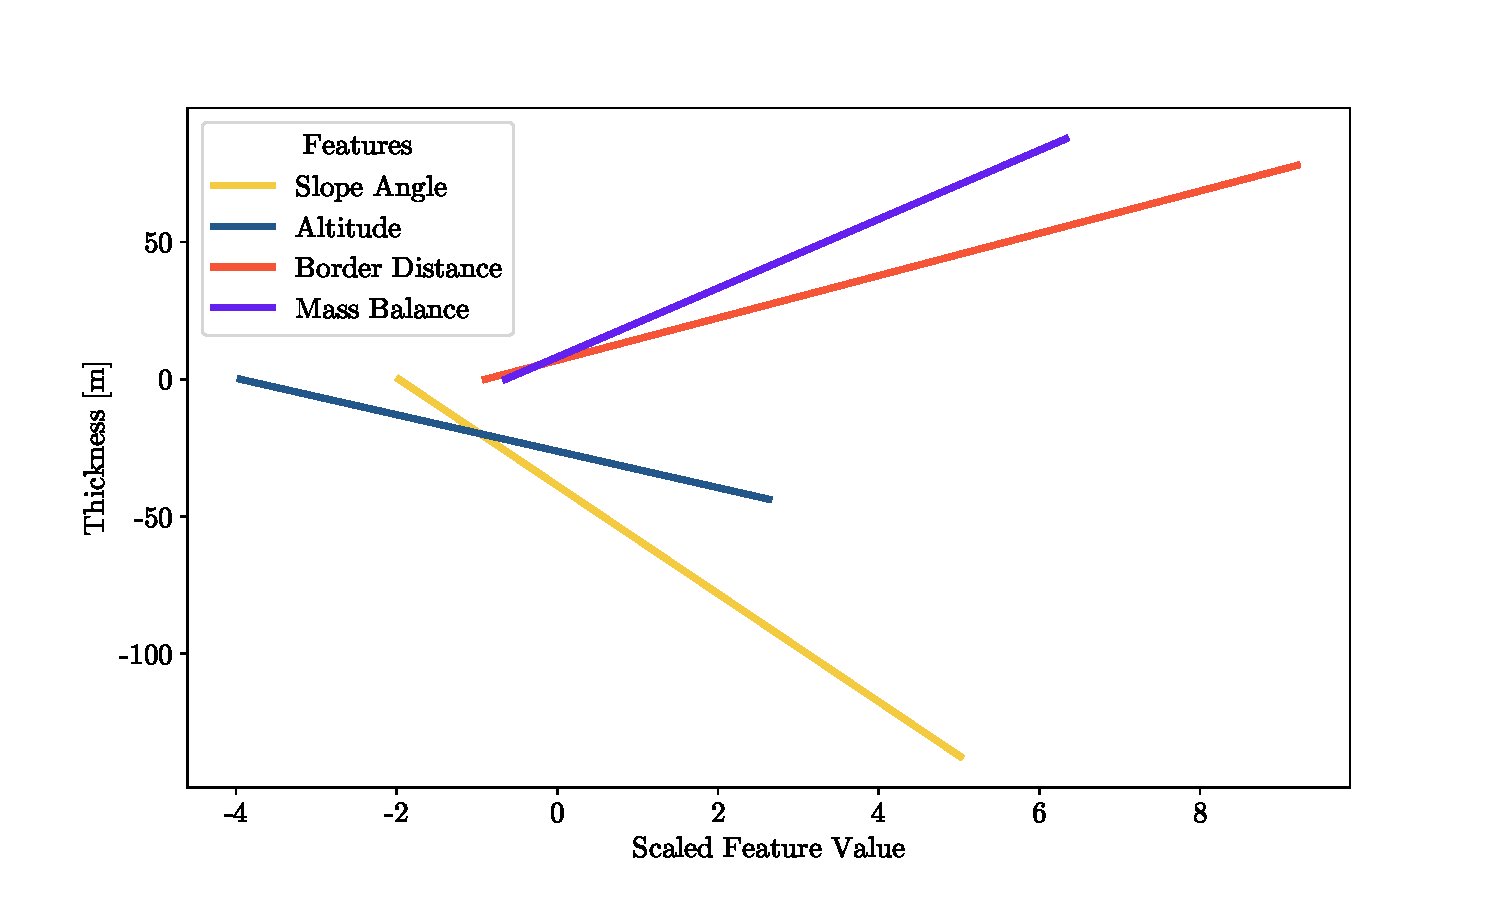
\includegraphics[width=1.\textwidth]{figures/LR_pdp.pdf}
	\caption{Linear Regression partial dependence plots: representation of the change in Ice Thickness compared to the change in the value of the features. Features values are scaled according to Eq. \ref{eq:scale}}
	\label{fig:lr-pdp}
\end{figure}

\section{Random Forest Regression}\label{rfr}
The same process of using different sub-samples to train the algorithm and testing its performance used in the linear regression case, has been used for the random forest algorithm. This is particularly important for random forests because they are very prone to over-fitting. Especially the parameters determining the maximum tree depth, and the one determining the minimum number of samples required to split the tree, are those which had to be carefully adjusted in order to maintain a good balance between the model performances, and its inability to generalize for samples not used to train it. The maximum tree depth parameter has been tuned in order for all the nodes to be expanded, until all the samples at the node would have the same label, or until the minimum sample necessary for the tree to split would be reached. The minimum sample required for the tree to split has been set to 5\% of the number of samples present in the training data-set.  

\subsection{Score and volume spread}\label{rfr-score}

\begin{figure}[!tp]
	\centering		  
	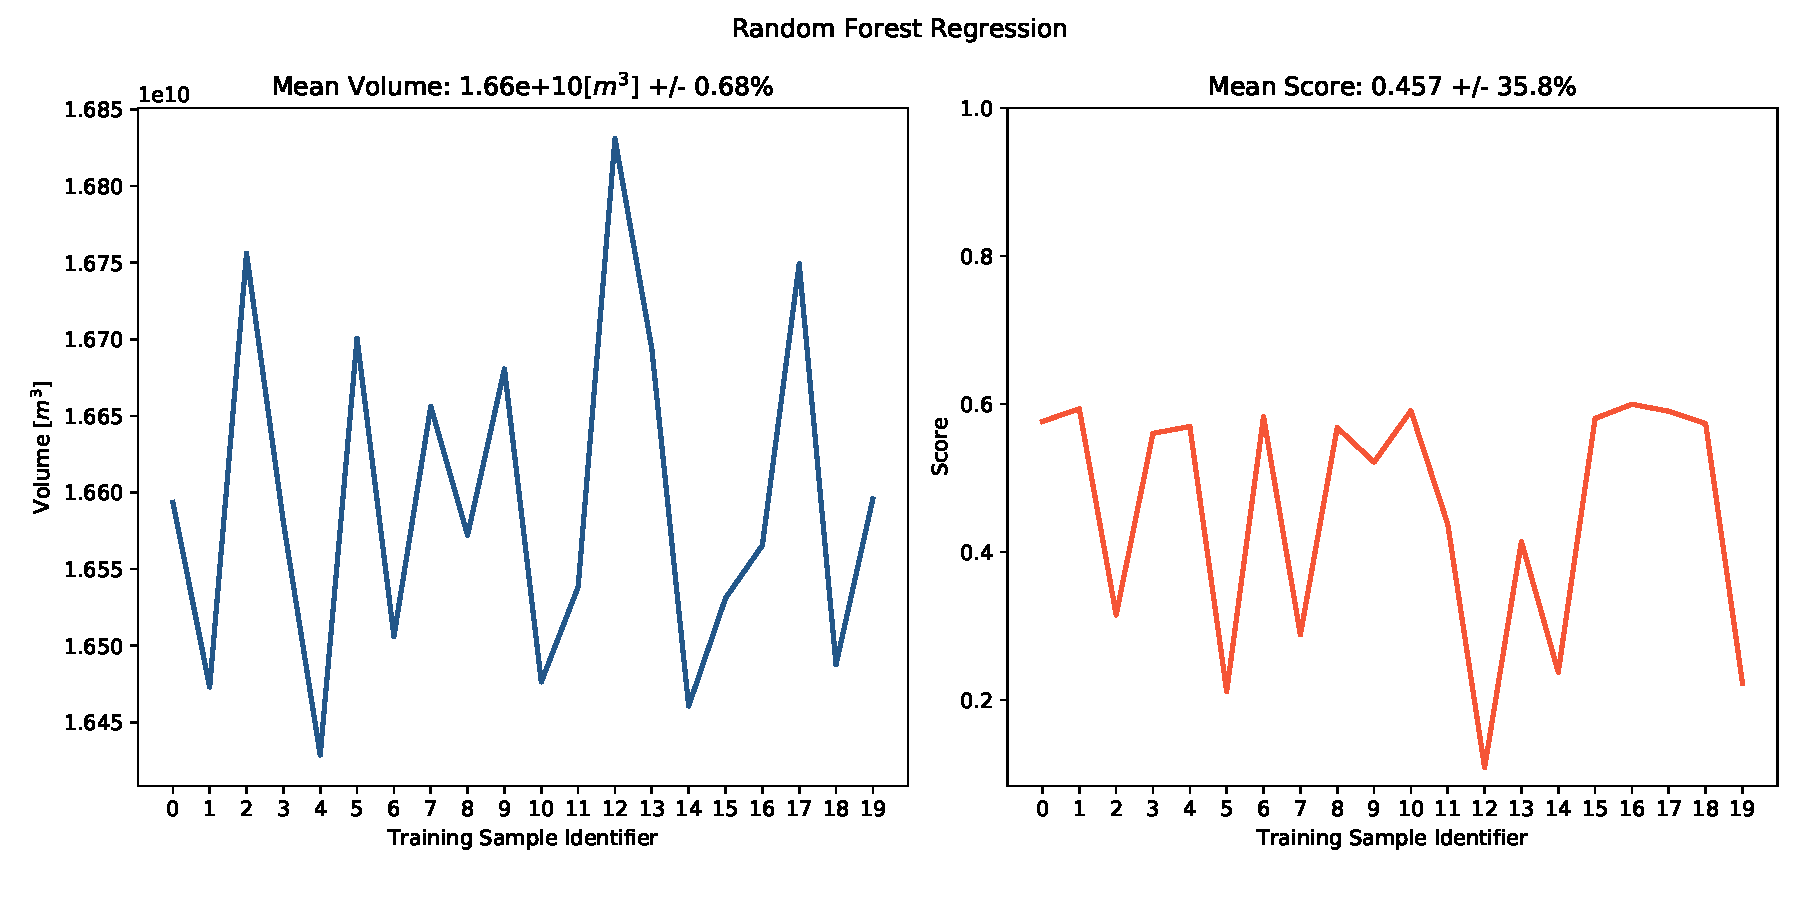
\includegraphics[width=1.\textwidth]{figures/RFR_score.pdf}
	\caption{Random Forest Regression: Volume and score values of the model after training it with 20 different sub-sample of data. On the x-axis each number identifies a different sample of data. On the left the total volume of the alpine glaciers present in the GlaThiDa. On the right the $R^2$ coefficient for values left out of the training sample.}
	\label{fig:rfr-score}
\end{figure}

Figure \ref{fig:rfr-score} shows the volume and score changes for 20 different sub-samples used for training the linear regression algorithm. 

It must be reminded that as the name of the algorithm suggests, part of its training process is random, due to the random processes used to create the different trees of the forest (see section \ref{random-forest}). This means that training the model again could produce slightly different results then the ones shown in Fig. \ref{fig:rfr-score}.

The score shown seems to be dependent on the sample used for training. This could mean that the model has been over-fitted, but it's also a common characteristic of random forest algorithms (\citet{RandomForest2018}). For some samples the score is around 0.6 but it gets as low as almost 0 for sample 12. As for the linear regression case low scores are registered for samples 5, 14 and 19 but also for samples 8, and 12. 
The model trained with all the data available from GlaThiDa reached a score 0.57, which is the highest of all the models tested.


\begin{figure}[!tp]
	\centering		  
	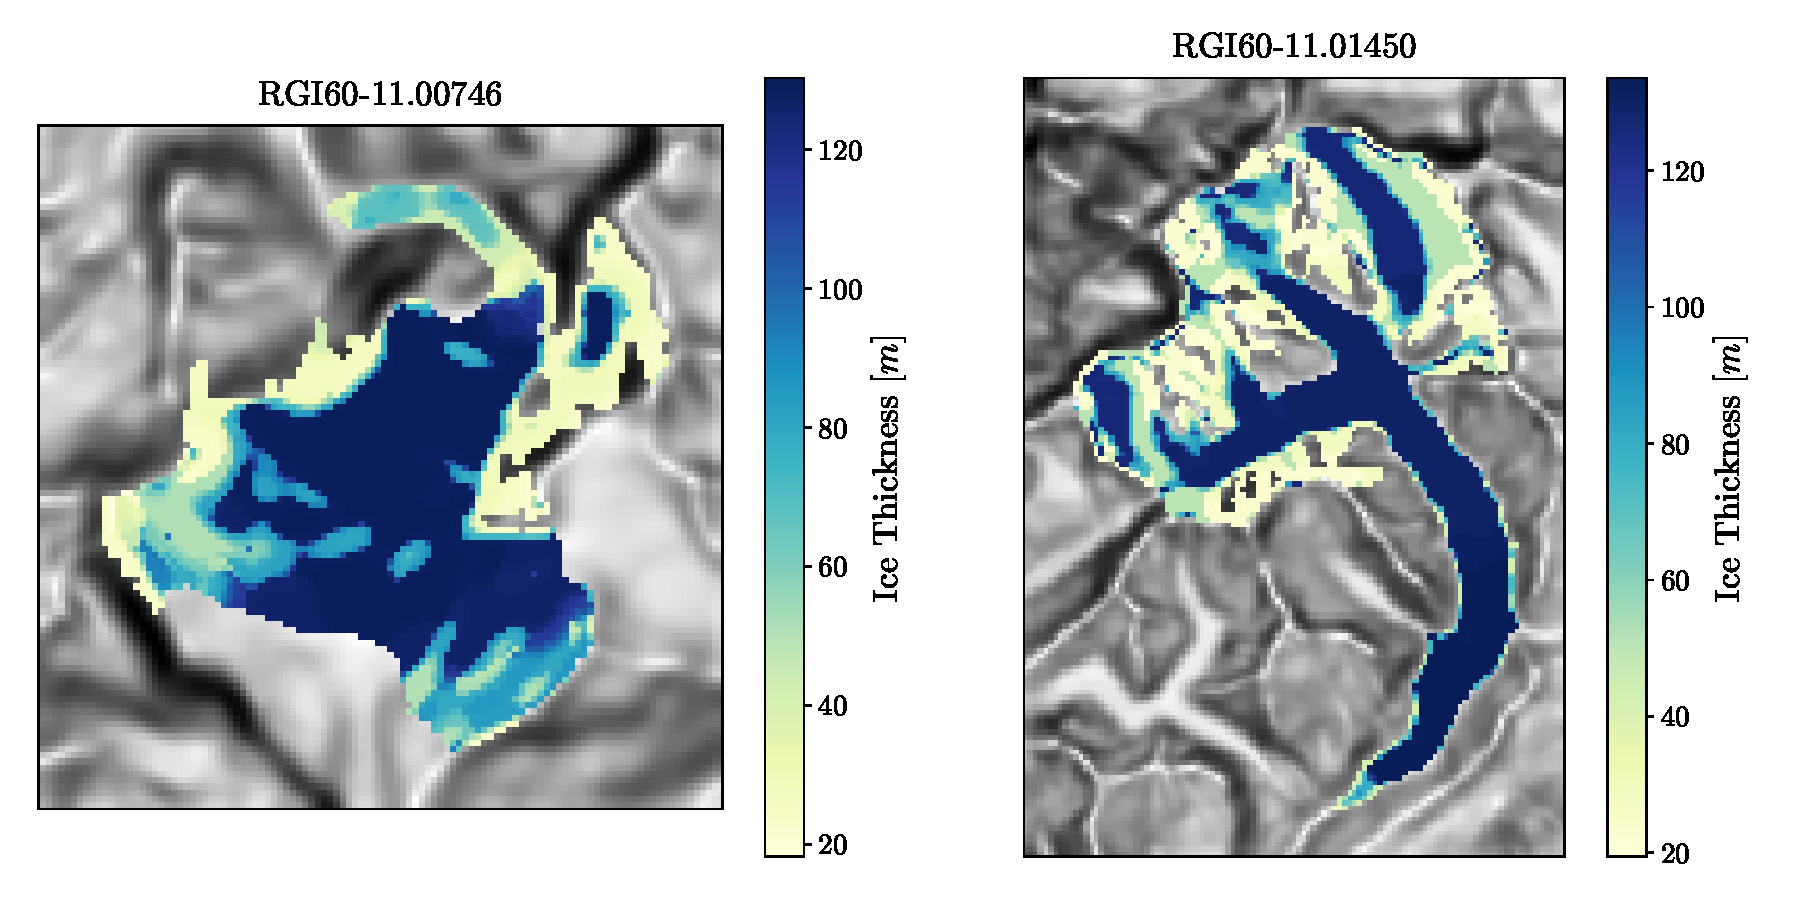
\includegraphics[width=1.\textwidth]{figures/RFR_thick_map.pdf}
	\caption{Random Forest Regression: Ice thickness distribution for two glaciers on top of the terrain slope angle. On the left, one of the glaciers used to train the model. On the right, one of the glaciers outside those used to train the model.}
	\label{fig:rfr-map}
\end{figure}

Contrary to the score values, the volume spread is not that high. The model seems to fail to correctly predict specific ice thickness, and its score is influenced by the sample chosen for training. This does not however seems to influence the total volume predicted for the glaciers for which this volume has been computed.

In Fig. \ref{fig:rfr-map} the ice thickness distribution predicted by the model for two different glaciers is shown. The ice thickness distribution seems to be distributed in a rather discontinuous way, with large areas of the glaciers having relatively high but almost constant ice thickness values. 

The total volume for the alps computed with the random forest regression model is $9.96 \times 10^{10}m^3$, which is 22.1\% lower than the volume predicted by \citet{Farinotti2019}.

\subsection{Features Importance}\label{rfr-features}

As for the linear regression model, random forest regression allows for a direct way of computing how influential each feature is at making predictions. This is computed as the total decrease in node variance (see section \ref{random-forest}) (weighted by the proportion of samples reaching the node), averaged over all trees in the ensemble. This is a very convenient way of determining the importance of the features, but it has been found biased in some cases (\citet{RandomFBias2007}). For this reason performing a permutation importance test on the model, can help to confirm the results obtained from the variance reduction method. 

Figure \ref{fig:rfr-heatmap} shows the coefficients deriving from the permutation analysis on the left, and the feature importance deriving from the variance reduction on the right. Both are calculated using the models trained with the different training samples already used for the score analysis. The feature importance heatmap on the right predicts the slope angle to be the most important of the features. In fact it computes it to be on average 1.6 times more important than the mass balance in making predictions. Altitude and distance from the border seem to be of almost no relevance in making predictions for both the methods used. However the permutation importance points at the mass balance as the most important feature. The difference in permuting the slope angle or the mass balance isn't as pronounced as showed by the variance reduction method. The values for the permutation importance of mass balance and slope angle are in fact very similar.

\begin{figure}[!tp]
	\centering		  
	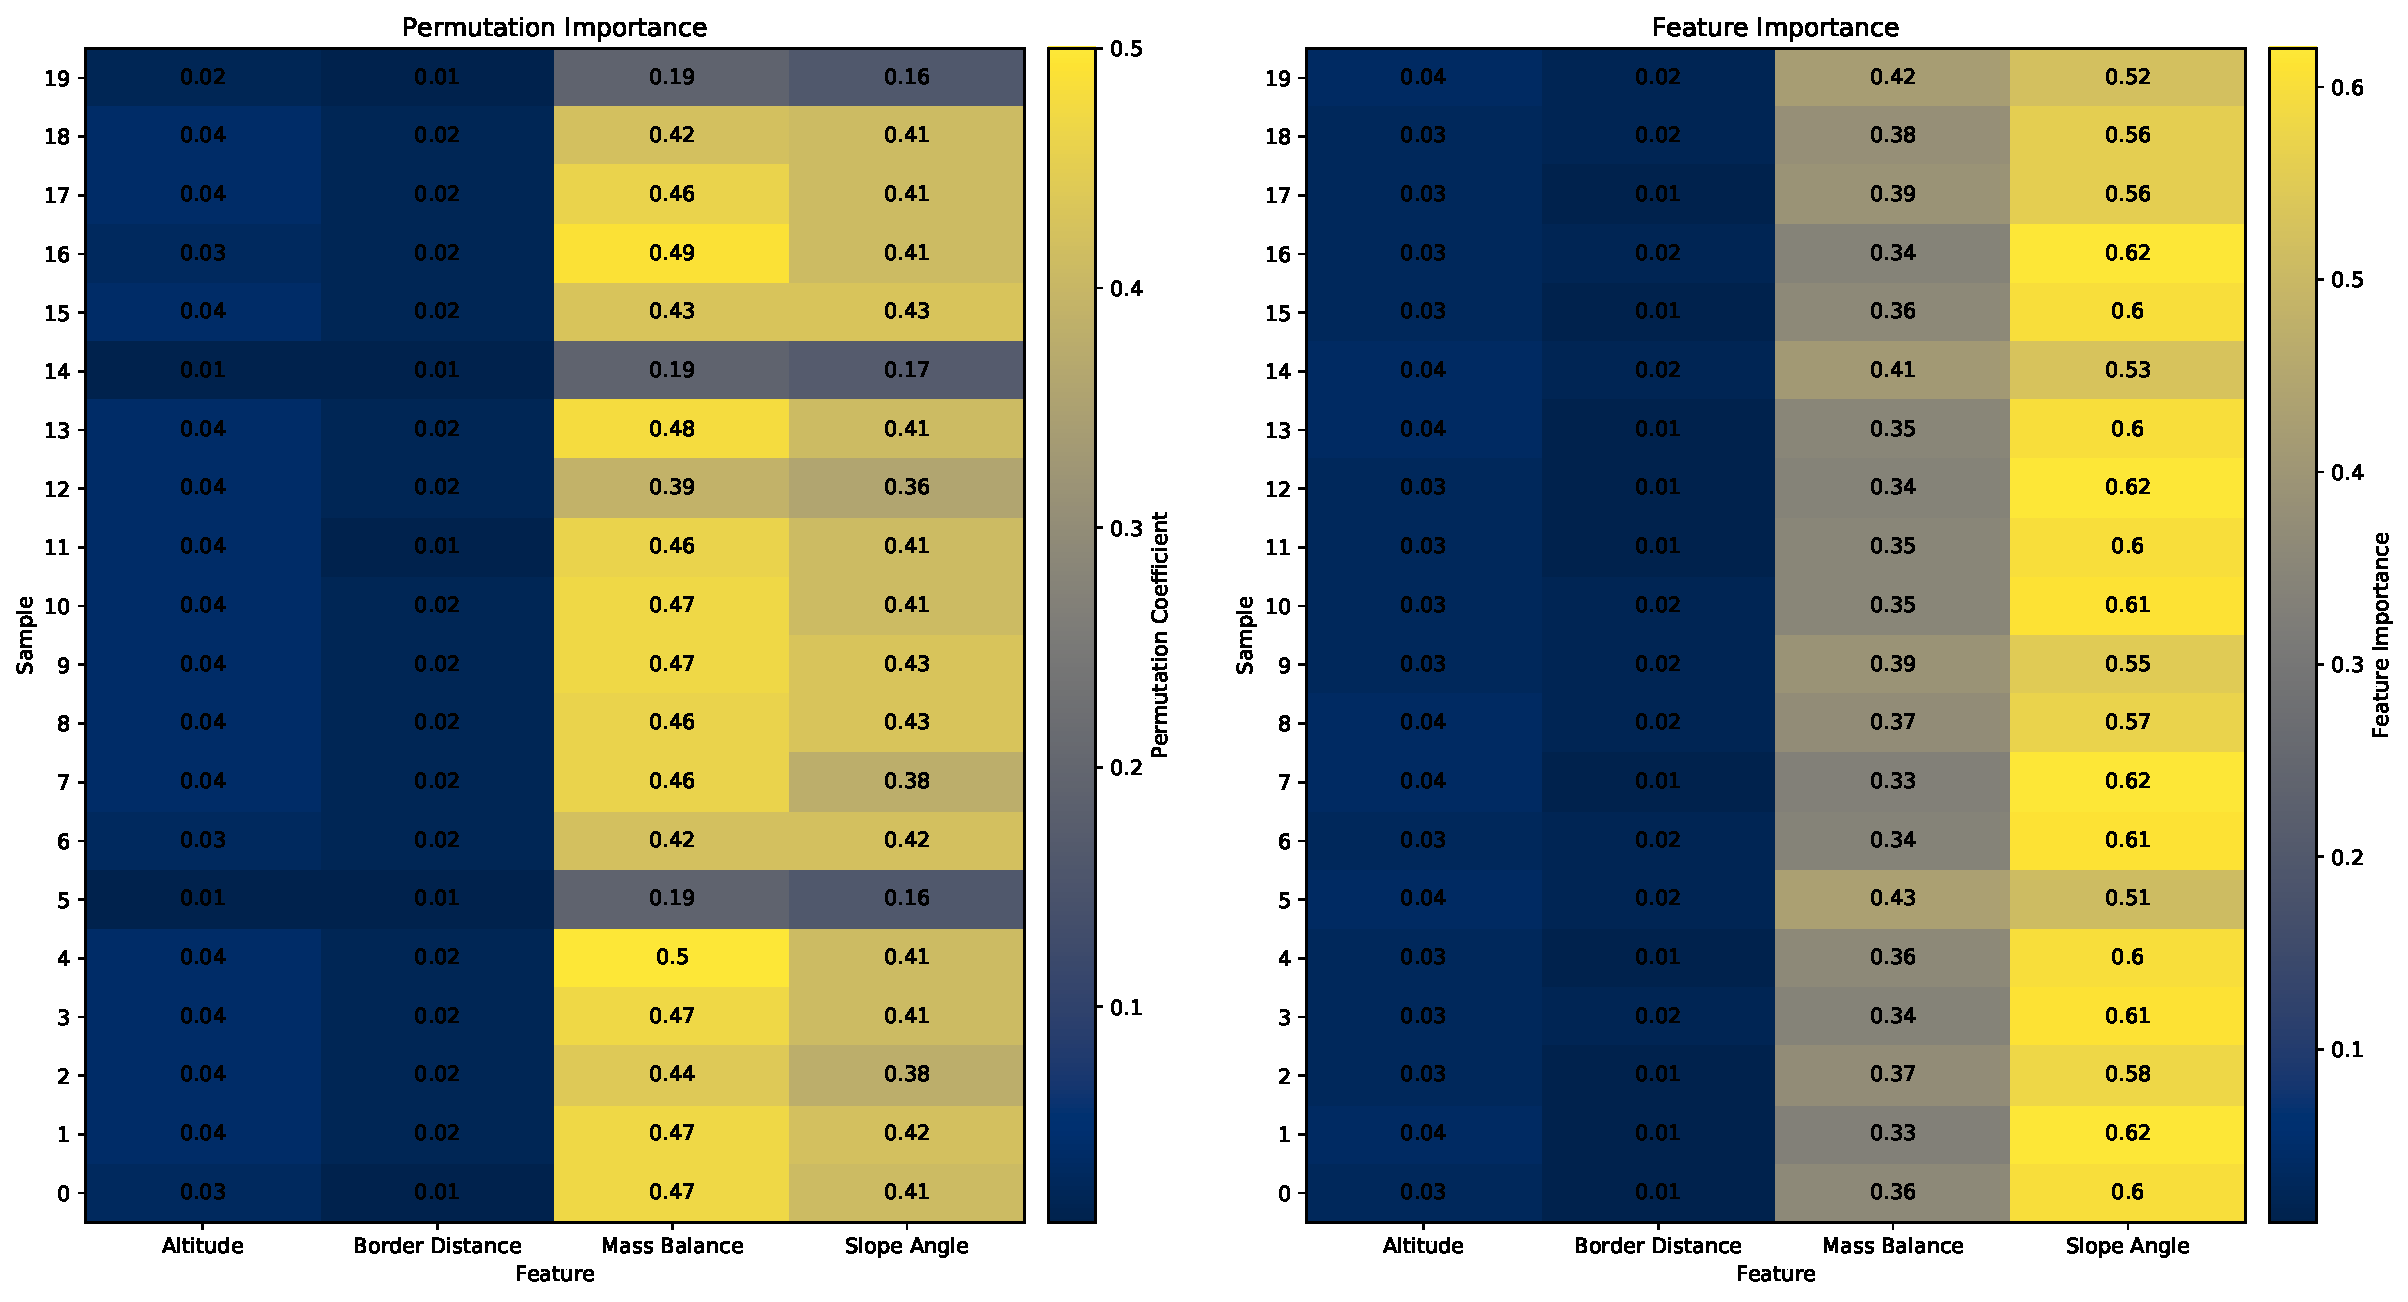
\includegraphics[width=1.\textwidth]{figures/RFR_heatmap.pdf}
	\caption{Random Forest Regression feature importance heatmaps: On the left the permutation coefficient; on the right the feature importance from the variance reduction method. Each row in the figure represents a sub-sample of the data used to train the algorithm. Each column represents respectively the permutation coefficient(left) or the variance reduction(right) value for the considered feature.}
	\label{fig:rfr-heatmap}
\end{figure}

Fig. \ref{fig:rfr-pdp} shows the change in thickness value for changes in values of the features. Once again, feature values are scaled according to Eq. \ref{eq:scale}. Immediately one sees that the change in ice thickness is not linearly dependent from the change in feature value. All the lines don't look continuous and present clear steps marking the change in ice thickness. This is partly due to the possible abrupt change in feature value, but it is mostly a natural effect of the sharp splits happening in the node of a decision tree.  The mass balance has a change in its slope going from increasing to decreasing around 0 and then increasing again around 1.8. The slope line has a sudden pick and changes from decreasing to increasing just below 0. The altitude also is slightly non monotonic between -1 and 0 while the border distance is always monotone. 
\begin{figure}[!tp]
	\centering		  
	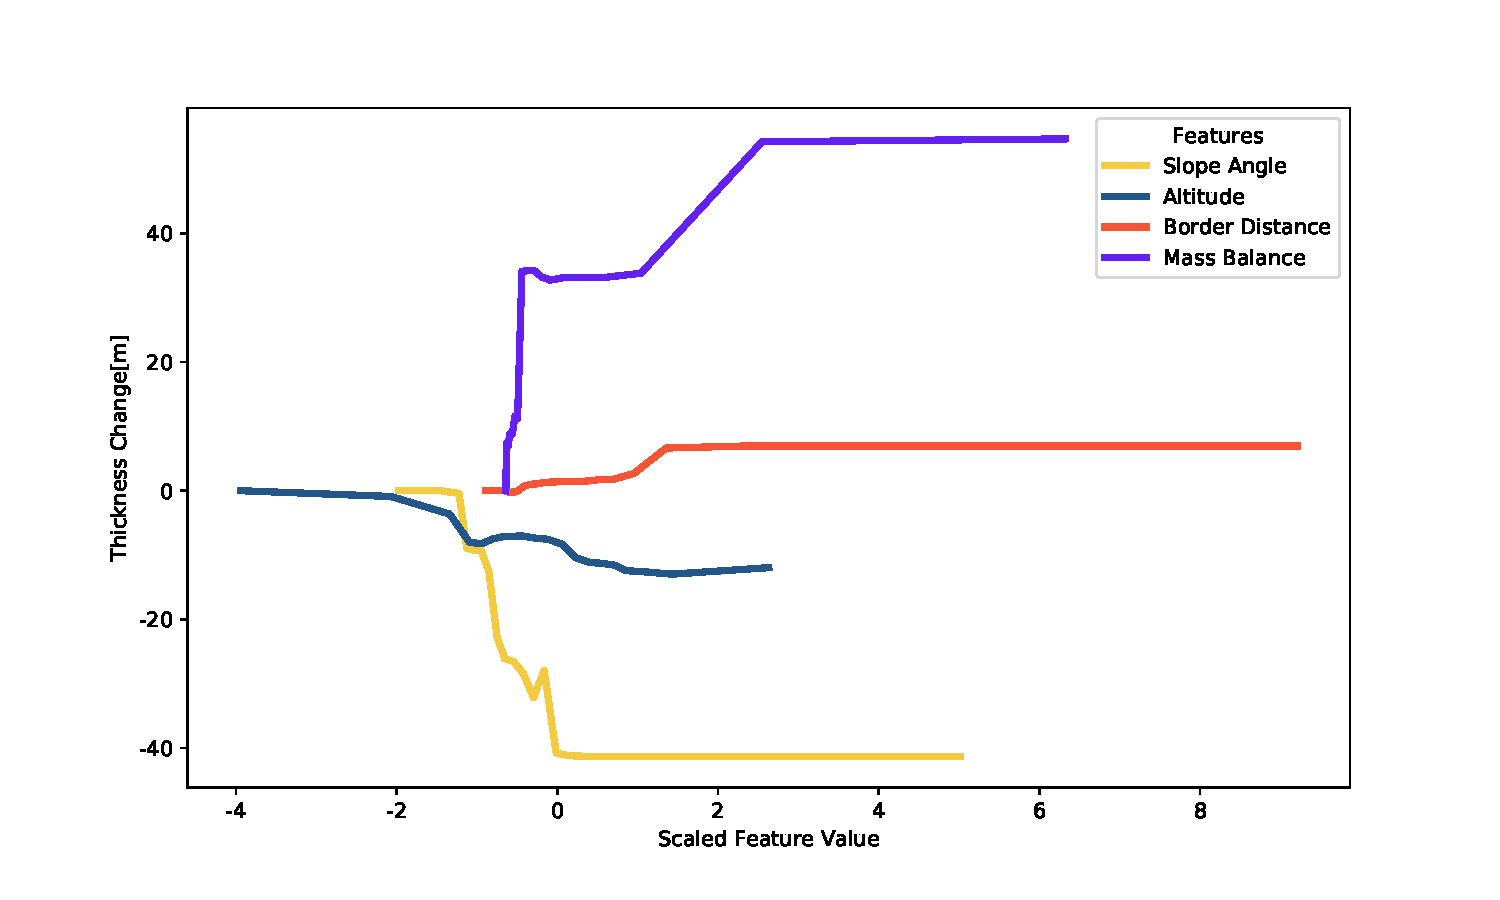
\includegraphics[width=1.\textwidth]{figures/RFR_pdp.pdf}
	\caption{Random Forest Regression partial dependence plots: representation of the change in Ice Thickness compared to the change in the value of the features. Features values are scaled according to Eq. \ref{eq:scale}}
	\label{fig:rfr-pdp}
\end{figure}

Fig. \ref{fig:rfr-pdp} also is in accordance with the feature importance analysis showed in the heatmaps of Fig. \ref{fig:rfr-heatmap} as the altitude and border distance seem to lead to very small changes in the ice thickness prediction. Looking at the partial dependence plots, it also seems like the slope leads to a change in ice thickness up until the scaled value reaches 0 (around $18^{\circ}$ angle). After this value the ice thickness prediction doesn't change. The maximum range of ice thickness change achieved by the slope angle is $40m$. For the mass balance there seem to be a change in ice thickness prediction throughout the whole range of its values up until scaled values just below 3. The steepest changes happen for values below 0. Its range in changes in ice thickness is almost $60m$ which is higher than the changes attributed to the slope angle.


\section{Support Vector Regression}\label{svr}
Support Vector Regression is the last model for which the results are presented here. The training process for this algorithm is notably slower compared to the linear regression and the random forest. However it is the model which reached the highest average score between the ones used. 

\subsection{Score and volume spread}\label{svr-score}

\begin{figure}[!tp]
	\centering		  
	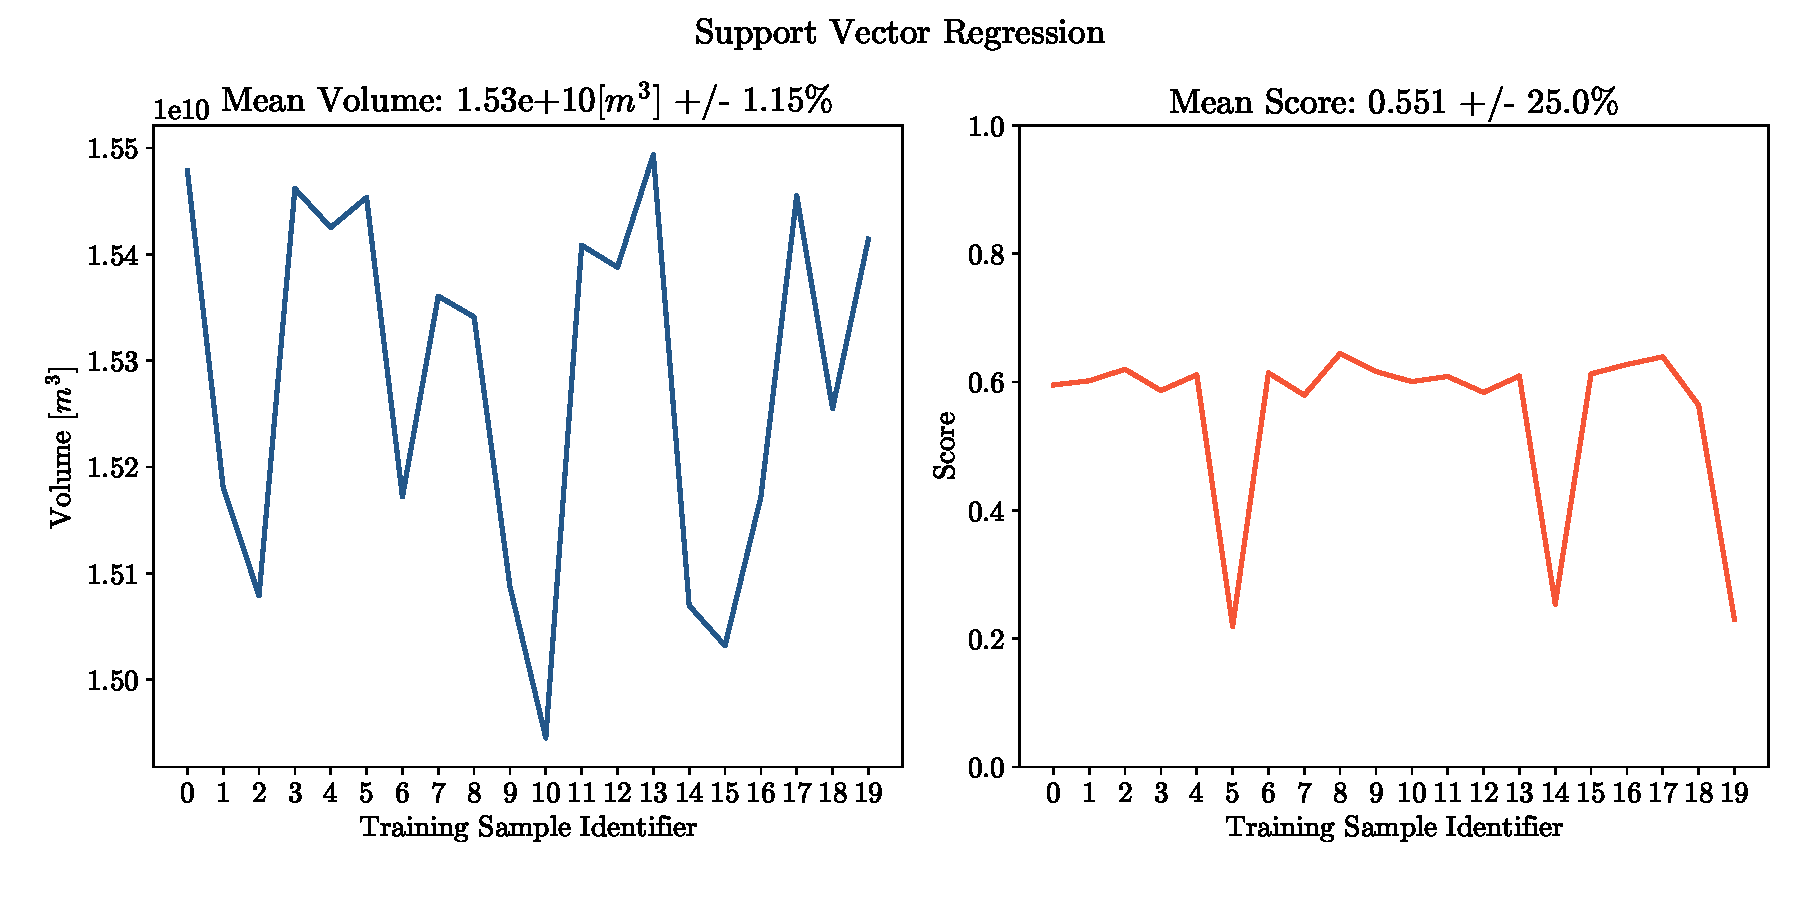
\includegraphics[width=1.\textwidth]{figures/SVR_score.pdf}
	\caption{Support Vector Regression: Volume and score values of the model after training it with 20 different sub-sample of data. On the x-axis each number identifies a different sample of data. On the left the total volume of the alpine glaciers present in the GlaThiDa. On the right the $R^2$ coefficient for values left out of the training sample.}
	\label{fig:svr-score}
\end{figure}

Fig. \ref{svr-score} shows on the left the volume spread for the alpine glaciers with ice thickness observations, and on the right the score of the model as defined in \ref{eq:score}. Each of the different values represent a model trained with a different sub-sample of data, the same sub-samples already used for the linear regression and random forest regression analysis.

The score shows a very similar pattern compared to the one shown from the linear regression model (see Fig. \ref{fig:lr-score}). Samples 5, 14 and 19 present a drop in the score achieved, exactly as already shown for the linear regression case. The average score however is higher reaching 0.55 on average and it is around 0.6 for most of the sub-samples used to train the model.
The value of the score for the model trained with all the data available from GlaThiDa is 0.45, which means that less than 50\% of the ice thickness variance is explained by the model. 

The volume spread on the left of the figure shows a dispersion around 1.15 and an average total volume of $1.53 \times 10^{10}m^3$. This is the lowest of all the models considered so far. 
Looking at Fig. \ref{fig:svr-map}, the ice thickness distribution for the glacier RGI60-11.01450 immediately looks strange. The ice thickness for most of the glacier seem to be in the order of 75$m$ with much higher values only reached in the very bottom part of it. It seems that the model is actually predicting a constant ice thickness for most of the glacier. This is of course not a desirable result as ice thicknesses are presumed to change throughout the surface of the glacier. The same behavior is not visible in the left glacier which shows different ice thicknesses uniformly distributed all over the glacier surface. Notice that the left glacier is one used to train the model, while the right one isn't.

The total volume of ice for the alpine glaciers predicted by the support vector machine is $9.58 \times 10^{10}m^3$, which is the lowest of all the models and 25\% lower than the volume predicted by \citet{Farinotti2019} with their ensemble model.

\begin{figure}[!tp]
	\centering		  
	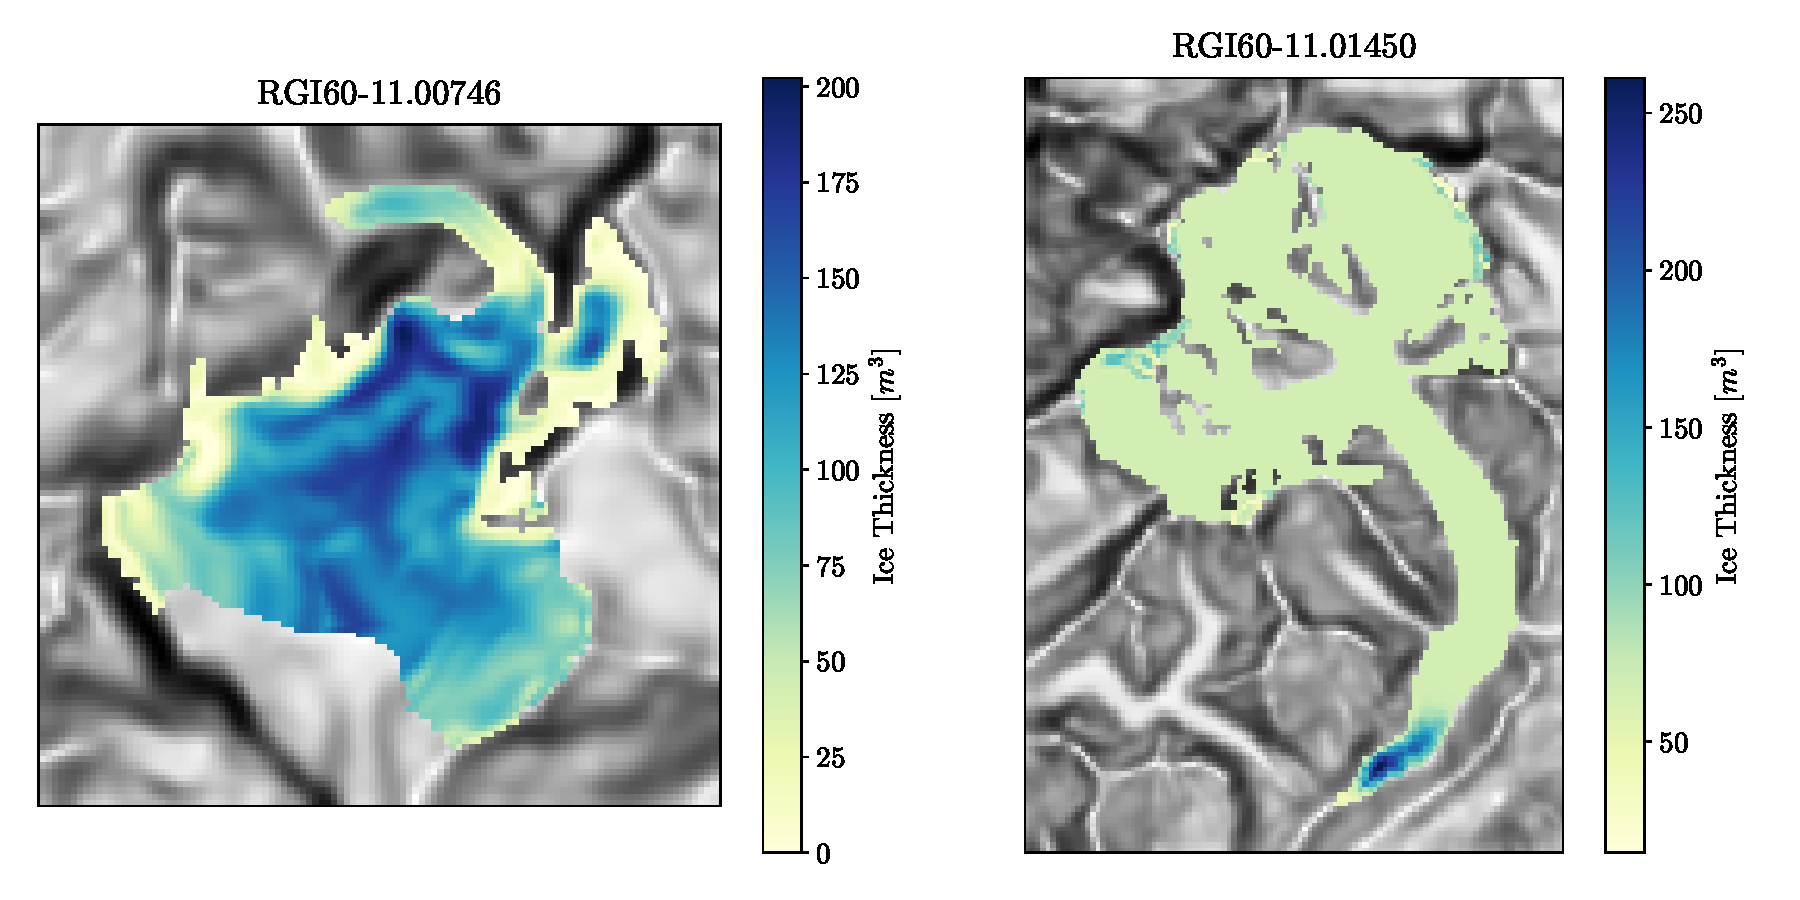
\includegraphics[width=1.\textwidth]{figures/SVR_thick_map.pdf}
	\caption{Support Vector Regression: Ice thickness distribution for two glaciers on top of the terrain slope angle. On the left one of the glaciers used to train the model. On the right one of the glaciers outside those used to train the model.}
	\label{fig:svr-map}
\end{figure}

\subsection{Features Importance}\label{svr-features}
Unlike linear and random forest regression, support vector regression doesn't have a simple way of computing the influence each feature has in making a prediction when using a non-linear kernel to transform the features. In order to analyze which features are the most important, one needs to recur to indirect methods such as the permutation importance.

\begin{figure}[!tp]
	\centering		  
	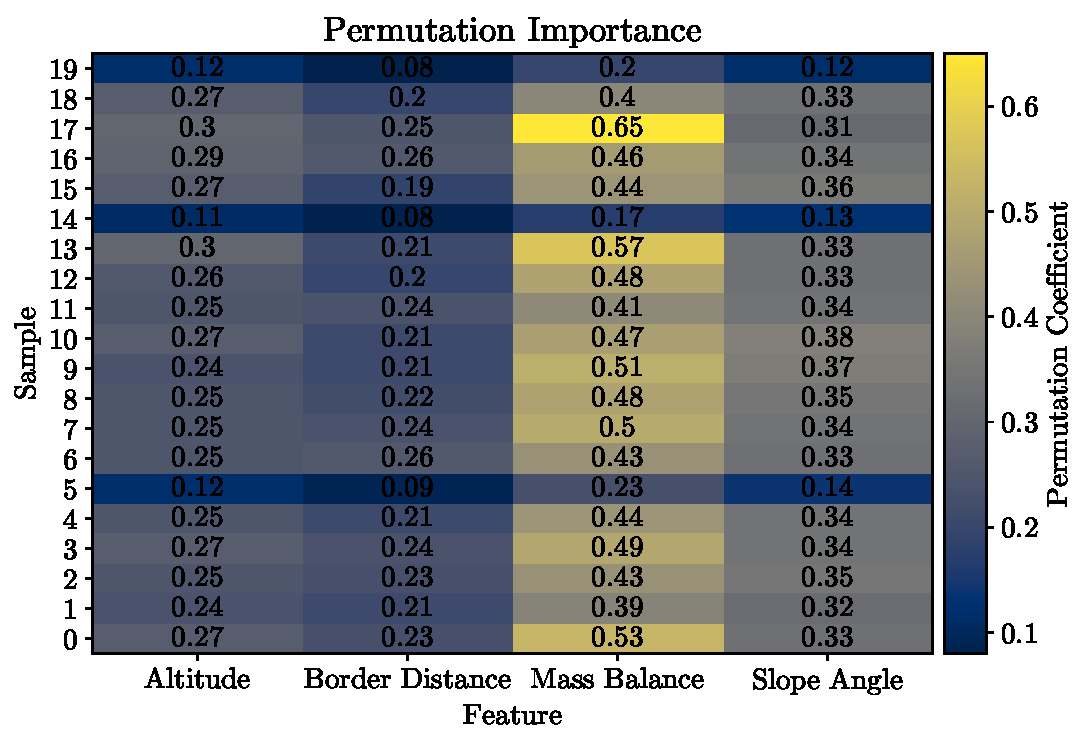
\includegraphics[width=0.8\textwidth]{figures/SVR_heatmap.pdf}
	\caption{Support Vector Regression feature importance heatmap: each row in the figure represents a sub-sample of the data used to train the algorithm. Each column represents the permutation coefficient value for the considered feature.}
	\label{fig:svr-heatmap}
\end{figure}

In Figure \ref{fig:svr-heatmap} the coefficients for the permutation importance (section \ref{permutation}) for all the models trained with the 20 different sub-ample of the data are shown. Once again the sub-samples with the lowest score registered (see Fig. \ref{fig:svr-score}), sub-samples 5, 14 and 19 are in general the ones displaying a lower value of permutation importance showing a dark blue line throughout the whole heatmap. Apart from those sub-samples, the linear mass balance above the point is the feature with the highest permutation importance even though values vary from 0.65 to 0.39. The second highest permutation importance values are those of the slope angle. In general then the most important features for the support vector regression model are the same as those of the random forest regression model. However the permutation coefficients of altitude and distance from the border are also comparable to those of the slope angle and they are also very close to each other, with the altitude seeming to play a bigger role compare to the border distance. All the features in general seem to play a role in the model final prediction. 

To complete the analysis of how the features influence the prediction of the support vector regression, Fig. \ref{fig:svr-pdp} shows the change in thickness value depending on changes in feature value. Again, the non-linear relation between the two is evident in this chart.  None of the curve is monotone and for each feature the ice thickness seems to increase or decrease depending on the value of the specific feature. Mass balance and slope angle drive the largest ice thickness changes looking at the range of those changes reached by those features curves. For feature values between 2 and 1 however the rate of change in ice thickness is similar between the altitude and slope angle, meaning that both these features compete in determining the ice thickness for those range of values. The same thing happens for values between around -0.5 and around 1.8 for the border distance and the linear mass balance, where again the two seem to compete in determining the predicted ice thickness.
\begin{figure}[!tp]
	\centering		  
	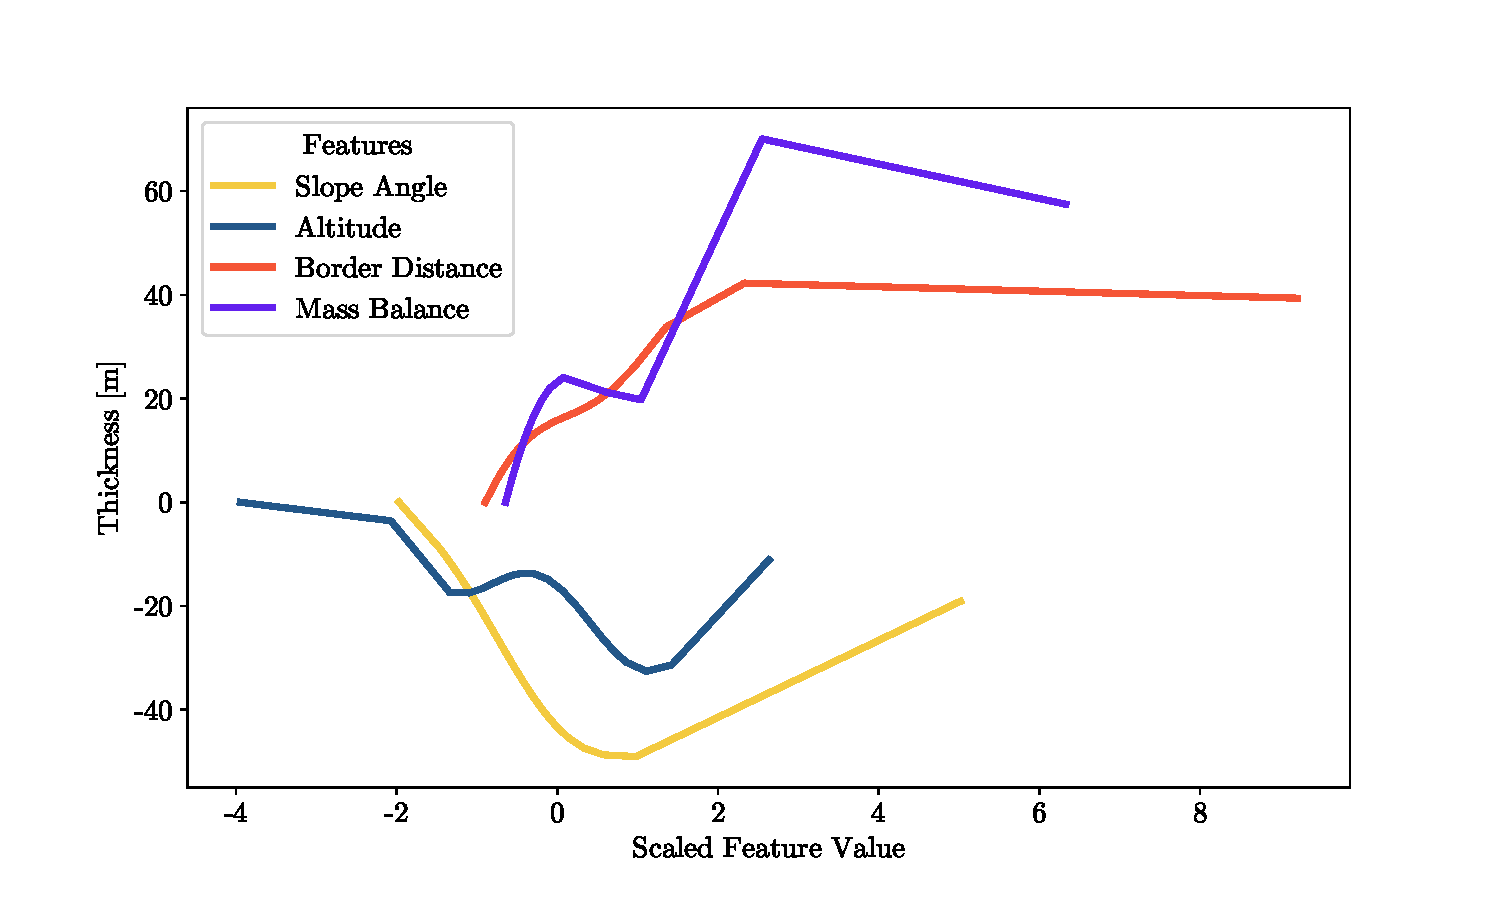
\includegraphics[width=1.\textwidth]{figures/SVR_pdp.pdf}
	\caption{Support Vector Regression partial dependence plots: representation of the change in Ice Thickness compared to the change in the value of the features. Features values are scaled according to Eq. \ref{eq:scale}}
	\label{fig:svr-pdp}
\end{figure}

This also seems to be in accordance with the analysis obtained with the permutation importance coefficients (see Fig. \ref{fig:svr-heatmap}). All features in fact seem to have some relevance in predicting the ice thickness at least for some of their value ranges. Mass balance and slope angle however seem to be more relevant throughout all their value ranges and also lead to a larger change in ice thickness, when looking at the minimum and maximum ice thickness change reached by their extreme values. 


% ==== SECTION 1 ===============================================================
%\section{Some Important Things to Know}\label{3sec:1}
%
%It is important to differentiate between \emph{facts} and \emph{interpretations}
%and between \emph{your contributions} and \emph{those of others}! Facts and
%your contributions are part of this chapter. Interpretations and contributions
%of others should be rather part of the chapter Discussion.
%
%
%\subsection{Experimental Parts in the Chapter Results}
%Experimental details should only appear in the chapter Results to the
%extent necessary to ensure comprehension. Painstaking descriptions of
%instruments, analysis procedures, field conditions, etc., should be part of the
%chapter Methodology. However, absolutely necessary is information that shows
%the \emph{reliability} of the findings and the \emph{robustness} of an
%innovation (e.g., a new analysis technique).
%
%
%\subsection{Numerical Results or so-called Data}
%Results are more than simply numbers! They are tiny but unique
%\emph{messages}. Data should not only be made ``visible'' (e.g., in
%figures, such as in Fig.~\ref{fig:1}) but should also be made
%\emph{articulate}.
%
%
%\subsection{Order of Presentation}
%Use chapters and (sub)sections to separate, e.g., various topics,
%questions, and problems, or to separate measurements from calculations. 
%Arrange information in a consistent way, e.g., from simple to complex, from
%small to large (or vice versa in terms of scales: e.g., from
%synoptic-scale to micro-scale), from \emph{most important} (central) to
%\emph{least important} (peripheral). Arrange the material in order to maximize
%impact rather than sticking to a strict chronological order. Try to tell a story
%that consists of a beginning, followed by a gradual unfolding, and a
%``happy end''.
%
%
%\subsection{Cross-References}
%You can always refer to other parts of your thesis like in the following
%example: See chapter \ref{chap2} or section \ref{1sec:3} or
%Fig.~\ref{fig:1} or Table~\ref{tab:1} or equation~(\ref{2equ:1}).
%
%
%\section{Figure}\label{3sec:2}
%Figure \ref{fig:1} shows an example for an EPS figure with two panels. The
%topography of the Wipp Valley and Inn Valley is shown in Fig.~\ref{fig:1a}.
%Figure~\ref{fig:1b} shows the time series of potential temperature at two
%stations. In order to refer to a certain range of figure panels write, e.g.,
%Fig.~\ref{fig:1a}--\subref{fig:1b}.
%
%
%\begin{figure}[!tp]
%\centering
%\figuretopcapfalse
%\subfigure[][]{
%  \label{fig:1a}  
%  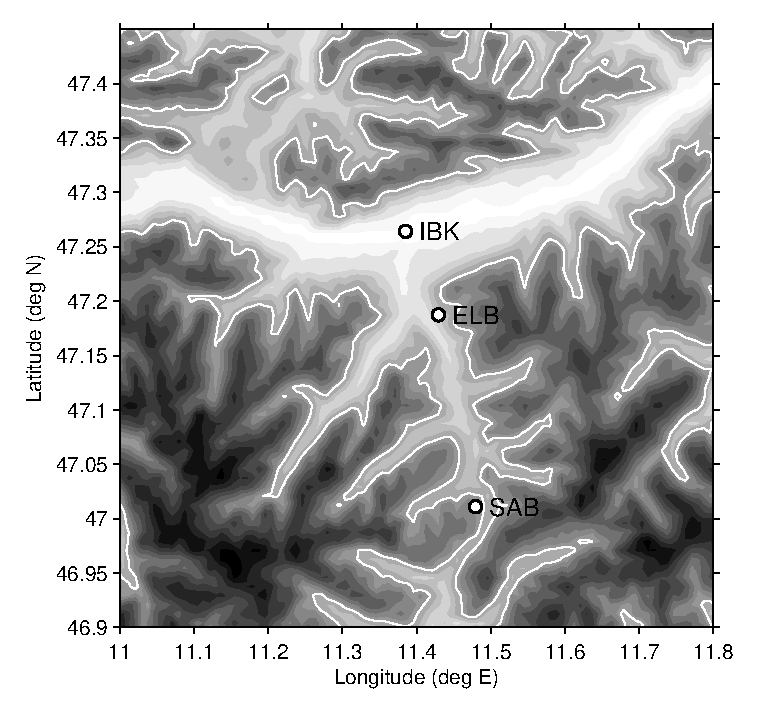
\includegraphics[width=0.48\textwidth]{figure_topo.eps}
%}
%\subfigure[][]{
%  \label{fig:1b}
%  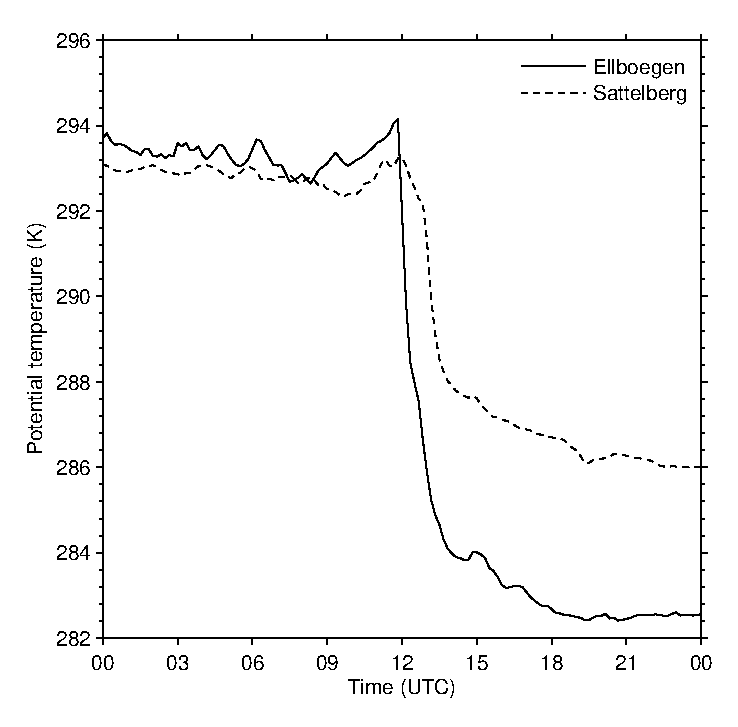
\includegraphics[width=0.47\textwidth]{figure_theta.eps}
%}
%\caption{(\subref{fig:1a}) Topographic map of the target area: Gray shaded
%elevations contours with increments of 200~m starting at 400~m~MSL and a white
%elevation contour line at 1600~m MSL. (\subref{fig:1b}) Time series of potential
%temperature (K) at Ellboegen (solid line) and Sattelberg (dashed line) from 00
%UTC 06 November to 00 UTC 07 November 1999. Labels in (\subref{fig:1a}) mark the
%location of Innsbruck (IBK), Ellboegen (ELB), and Sattelberg
%(SAB).}\label{fig:1}
%\end{figure}
%
%
%This template uses the \texttt{subfigure} environment with the option
%\texttt{FIGTOPCAP} to place the subfigure labels (\subref{fig:1a}) and
%(\subref{fig:1b}) at the top of the figure. However, since we want to have the
%caption at the bottom of figure, use \verb|\figuretopcapfalse|
%before the first \verb|\subfigure| command within the \texttt{figure}
%environment, otherwise the figure number produced by \verb|\ref| is wrong.
%
%
%\section{Table}
%Table \ref{tab:1} is an example for a table that consists of several
%rows and columns. Here, the \texttt{tabular} environment is used inside the
%\texttt{table} environment.
%
%
%\begin{table}[!htb]
%\centering
%\begin{footnotesize}
%\renewcommand{\tabcolsep}{4pt}
%\begin{tabular}{l p{3.5cm} l l l}
%\hline
%\hline
%Parameter & Code & Description & Units & Code\\
%\hline
%$g$ & \verb|$g$| & acceleration due to gravity&
%  m~s$^{-2}$ & \verb|m~s$^{-2}$| \\
%$T_d$ & \verb|$T_d$| & dew point temperature & $^{\circ}$C & 
%  \verb|$^{\circ}$C| \\
%$\mathbf{v} \cdot \nabla T$ & \verb|$\mathbf{v} \cdot| \verb| \nabla T$| &
%  temperature advection & K~s$^{-1}$ & \verb|K~s$^{-1}$| \\
%$\vec{v} \cdot \nabla T$ & \verb|$\vec{v} \cdot| \verb| \nabla T$| & 
%  temperature advection & K~s$^{-1}$ & \verb|K~s$^{-1}$| \\
%$\frac{\partial p}{\partial t}$ & \verb|$\frac{\partial p}|
%  \verb| {\partial t}$| & local pressure tendency & Pa~s$^{-1}$ &
%  \verb|Pa~s$^{-1}$| \\
%$p_0 \cos (kx - \omega t)$ & \verb|$p_0 \cos (kx| \verb| - \omega t)$| &
% wave expression & Pa & Pa \\
%\hline
%\end{tabular}
%\end{footnotesize}
%\caption{Some meteorological and mathematical parameters and expressions.}
%\label{tab:1}
%\end{table}
%
%
%\section{Figure and Table Captions}
%
%Figure and table captions \emph{must} contain all necessary information to
%understand the \emph{content} of the figure and table, without the need of
%additional text. Only in case of very complicated figures or tables, the caption
%may end with a remark such as ``See text for further explanation''. The
%\emph{interpretation} of the table or figure is not part of the caption, but
%should be given in the main text. In order to avoid repetitions, the phrase
%``As in Fig. xx, but for \dots'' is often used. Necessary information provided
%in the caption is a description of
%\begin{itemize}
%\item shown parameters together with units,
%\item date and time,
%\item contour intervals,
%\item location,
%\item line styles and markers,
%\item and others.
%\end{itemize}
%A list of figures and a list of tables at the beginning of the thesis (before
%chapter 1) is optional.
%
%
%
%\section{Title}
%
%The title of your science thesis should be kept as short as possible. It should
%represent an extremely compact summary of the thesis. The title should provide a
%clear and complete description of the topic and should contain many keywords
%(``what?'', ``how?'' and possibly ``why?''). The main title should not contain
%more than 10 words. An optional subtitle may be used if necessary (all together
%not more than 25 words). Important words and terms should be placed at the
%beginning of the title. Avoid unspecific expressions such as
%\begin{itemize}
%\item[] Investigation of ...
%\item[] Experiments on ...
%\item[] Results of ...
%\item[] Attempts to ...
%\end{itemize}
%Rather use expressions such as
%\begin{itemize}
%\item[] Influence of ... on ...
%\item[] Generation of ... with ...
%\item[] Dependence of ... upon ...
%\item[] Optimization of ... upon ...
%\end{itemize}
%Avoid technical abbreviations or acronyms and special symbols such as IR
%for infrared or $\theta$ for potential temperature.
%
%
%\section{Abbreviations and Symbols}
%Abbreviations (e.g., ECMWF) and symbols (e.g., $\vec{v}_g$) have to be
%defined, i.e. explained, at the place where the \emph{first} appear in the text.
%For example: The model was initialized with the operational analysis of the
%European Centre for Medium-Range Weather Forecasts (ECMWF). From the ECMWF
%fields of geopotential height we derive the geostrophic wind vector
%$\vec{v}_g$. The change of $\vec{v}_g$ with pressure $p$ reveals the thermal
%wind equation.
%
%A list of abbreviations and a list of symbols at the beginning of the thesis
%(before chapter 1) is optional.
%
%
%\section{Parameters and Units}
%
%Use italic letters for scalar quantities (e.g., $R$ and $g$), bold upright
%letters or arrows for vector quantities (e.g., $\mathbf{v}_g$ or $\vec{v}_g$)
%and sans-serif letters for tensors (e.g., $\mathsf{T}$). All this parameters
%should be written in mathematical mode (\verb|$ ... $|). Units should be
%written with normal upright letters (e.g., m~s$^{-1}$). Use spacing between
%numbers and individual units (e.g., $\phi=100$~W~m$^{-2}$). Less or no spacing
%is used between numbers and units in case of percent and degrees (e.g.,
%10\% and 5$^{\circ}$C). See also Table~\ref{tab:1} for further examples.
%
%
%\section{Footnotes}
%Do not use footnotes in an extensive way. Footnotes distract the reader from the
%main body of the document. Do not use footnotes for referring to literature,
%rather use the author-year citation system together with a bibliography (list
%of references) at the end of the thesis.